\chapter{Everyday use}
\label{ch:usage}

This chapter walks through the workflows you will run dozens of
times once the library is live: cataloging a new volume, searching
your collection, moving a volume, lending it out, taking it back,
and auditing what is on the shelves.

\section{The sidebar}\label{sec:navbar}

On a window at least 1024\,px wide, the navigation lives in a
\emph{sidebar}\index{sidebar} on the left of the page; it stays in
place while the page scrolls. Its entries come in groups separated by
a thin line: \textbf{Home}; then \textbf{Catalog}, \textbf{Locations}
and \textbf{Series}; then, for Librarians and Admins,
\textbf{Borrowers}, \textbf{Loans}, \textbf{Wish list},
\textbf{Labels} and \textbf{Proposals}; and, for Admins only,
\textbf{Admin}. The page you are on is shown in bold, with a coloured
bar on its left edge. The \textbf{Proposals} entry carries a badge
counting the proposals waiting for a decision (\texttt{99+} above 99;
chapter~\ref{ch:agents}).

The foot of the sidebar holds the language selector, the theme toggle,
and \textbf{Log out} (or \textbf{Log in} for an anonymous visitor).
Below them, the \textbf{Collapse menu} button narrows the sidebar to a
column of icons, which leaves more room for the page; hovering an icon,
or reaching it with the Tab key, shows its name in a tooltip, and the
Proposals badge becomes a small pill on the icon. The same button
expands the sidebar again. The browser remembers the choice: the next
page, and the next visit, open in the same state. The choice belongs to
the browser, not to the account --- another computer keeps its own.

\paragraph{On a phone or a narrow window.} Below 1024\,px the sidebar
is hidden and a slim bar stays at the top of the page, with the
\textbf{menu} button (three horizontal lines) and the mybibli logo.
The menu button opens the same navigation as a drawer that slides in
from the left over the dimmed page: same entries, same badge, and the
language selector, theme toggle and Log out (or Log in) at its foot;
it is never collapsed. Escape, a tap on the dimmed page, the close
button at the top of the drawer, or following one of its links closes
it. While the drawer is open, the page behind it neither scrolls nor
receives the keyboard, and a barcode scanner read is ignored rather
than typed into the scan field.

\paragraph{Light and dark theme.} The theme toggle switches the whole
interface between light and dark. The browser remembers the choice;
until you make one, mybibli follows the system setting of the device.
Printed pages are always light, whatever the theme on screen.

\section{The home page}\label{sec:home}

\begin{figure}[ht]
  \centering
  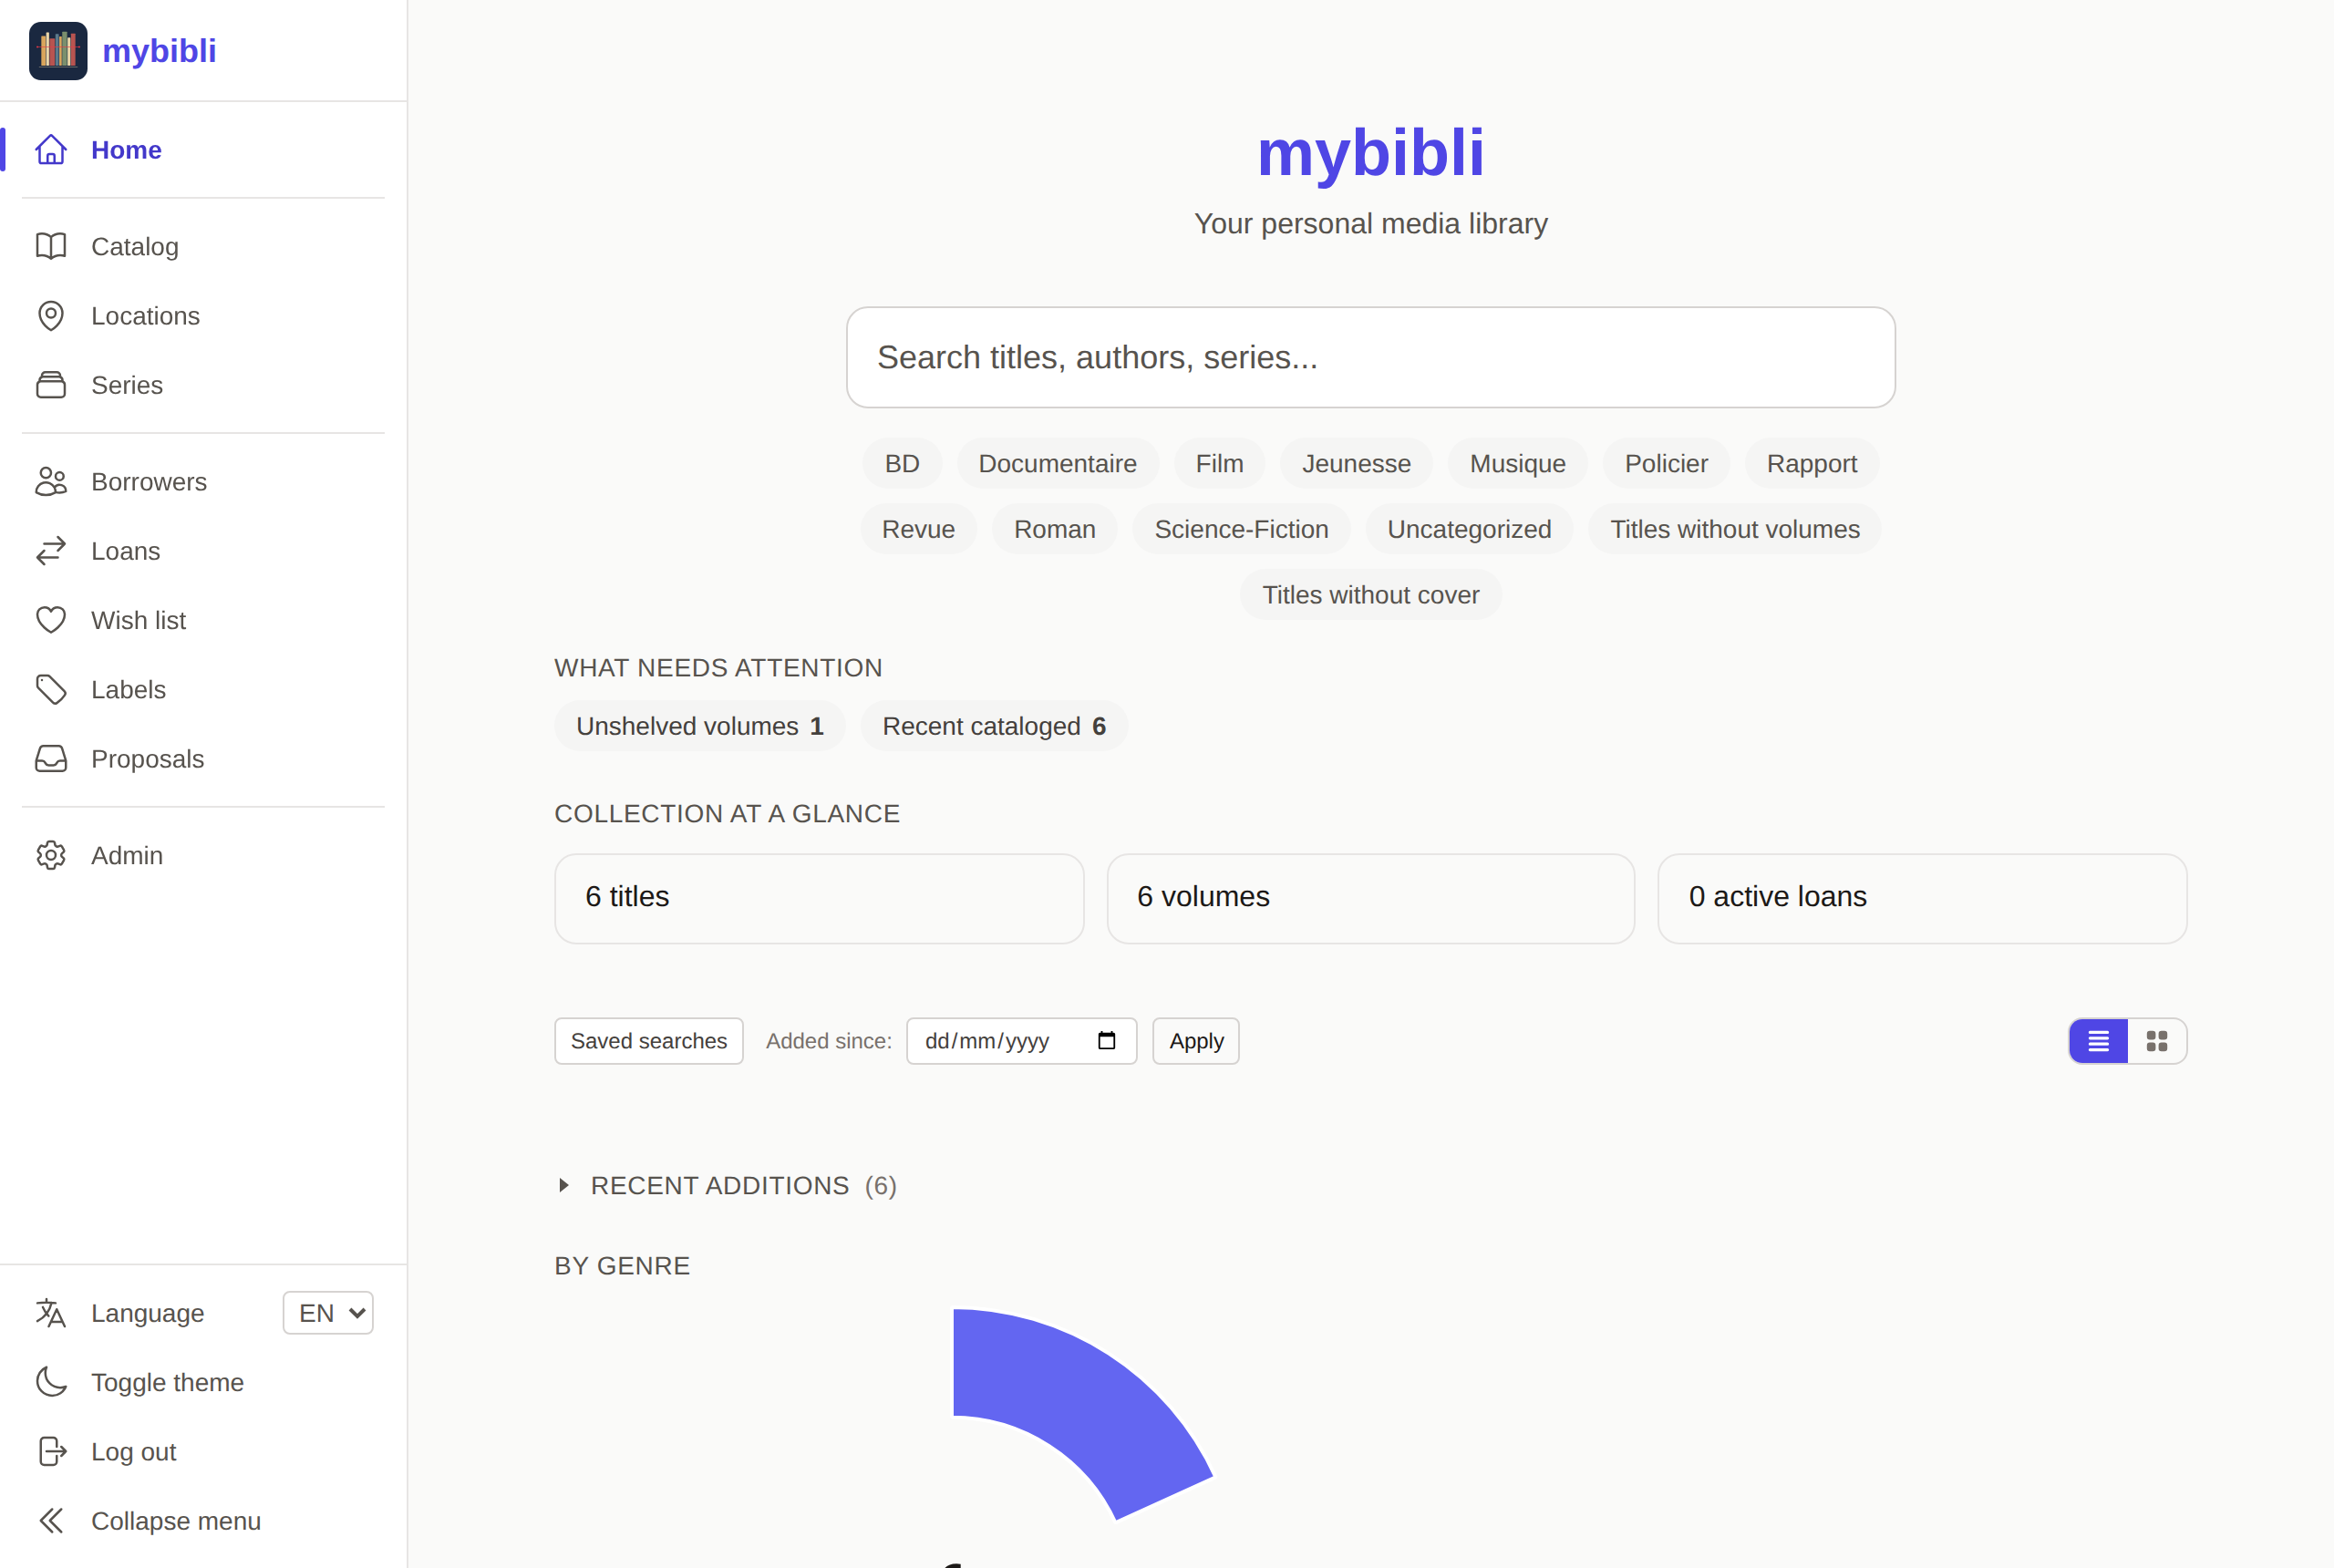
\includegraphics[width=0.95\textwidth]{01-home-desktop-en.png}
  \caption{The home page in a 1280\,px window, signed in as an Admin:
    the expanded sidebar on the left (language, theme and Log out at
    its foot, the collapse button below them), then the search bar,
    genre filter chips, the ``What needs attention'' counters and
    the ``Collection at a glance'' totals.}
  \label{fig:home}
\end{figure}

The home page is the dashboard. From top to bottom:

\begin{itemize}
  \item \textbf{Scan field.}\index{scan field} A focused input that
        accepts an ISBN, a V-code or an L-code. The scanner-guard
        layer routes the input to the right page depending on its
        prefix. An ISBN typed by hand may keep the hyphens or spaces
        printed on the book (\texttt{978-2-205-00121-1},
        \texttt{2 205 00121 3}): mybibli removes them and handles
        the bare ISBN-13, at scan as in the search.
  \item \textbf{Indicators row.} Recent additions, overdue loans,
        series with gaps, unshelved volumes — each click jumps to
        the filtered list.
  \item \textbf{Recent activity.} The last seven days of cataloging
        and returns. A title counts as \emph{recently cataloged} when
        the title itself, or one of its volumes, was added in those
        seven days (section~\ref{sec:added-since}).
  \item \textbf{Recent additions.} The titles that received something
        most recently --- the title itself or a new volume, whichever
        is later. They follow the \emph{List view} / \emph{Grid view}
        toggle of the catalogue below: in list view they appear as the
        same table (with its \emph{Added} column), in grid view as
        cards. Switching the toggle changes both at once, and the
        choice is remembered on the next visit.
\end{itemize}

\section{Cataloging a new title via barcode}\label{sec:catalog-scan}

\begin{enumerate}
  \item Focus the home-page scan field (it is selected by default
        on page load). Scan the ISBN / EAN-13 of the back cover.
  \item mybibli redirects to the catalog page, which displays a
        skeleton title with the barcode you scanned. A background
        task fires off requests against the metadata provider
        chain.
  \item Within a few seconds, the skeleton fills in: title,
        contributors, publisher, year, cover image. A small
        indicator confirms which provider resolved the title.
  \item Pick a \textbf{location}\index{location} from the dropdown
        (or scan the L-code of the destination shelf) and pick a
        \textbf{volume state}\index{volume state} (typically
        \emph{New}). Click \textbf{Add volume}.
  \item Print and stick a V-code label on the volume.
\end{enumerate}

If the metadata pipeline fails to resolve the ISBN, the title
appears with an \emph{Unresolved} badge. You can edit the title
fields manually and the volume is still created.

\begin{tip}
Cataloging in batches works best when the V-code sticker roll, the
scanner and the printer are all within arm's reach. Most of the time
is spent scanning, not waiting for mybibli — the metadata fetch is
asynchronous, so you do not have to wait for it to finish before
moving on to the next volume.
\end{tip}

\subsection*{Scanning a V-code that is already in use}
\label{sec:scan-existing-vcode}

A pile of books scanned in a hurry produces repeats. Since 1.23.0
mybibli tells them apart instead of answering every one with an error:

\begin{itemize}
  \item \textbf{A double read of the scanner.} The same code arriving
        twice within one second from the same scan field is read
        once: the second read is dropped silently and the field is
        cleared. This applies to every kind of code. The same code
        scanned again after that second is processed normally.
  \item \textbf{A V-code of the current title.} Scanning again the
        ISBN and the V-code of a book already catalogued (with no
        active location) creates nothing; an information message says
        \emph{``Label V0042 is already recorded for this title.''}
  \item \textbf{A V-code of another title.} The V-code is not moved
        and nothing is created. A warning names the title that holds
        it, with its ISBN when it has one, links to the volume page,
        and suggests scanning another sticker for the book in hand or
        opening the volume: from its page you can move it to the right
        title (section~\ref{sec:move-volume-title}).
  \item \textbf{A shelving that did not happen.} With an active
        location, scanning a V-code shelves the volume there. If the
        change could not be saved, or if the active location was
        deleted in the meantime, the message says the volume was
        \emph{not shelved} and what to do (scan the V-code again, or
        scan another L-code); a deleted active location is cleared.
\end{itemize}

\subsection*{Printing fresh label sheets}

Before printing a new sheet of V-code or L-code labels, check the
small line at the top of the catalog page (since 1.12.0, Librarian
and above): \emph{``Labels in use up to V0142~·~L0037 --- print new
label sheets starting after these numbers.''} The numbers include
items currently in the trash — a sticker that was ever printed and
stuck on a book is never proposed again, even if that volume was
deleted since.

\section{Searching the collection}\label{sec:search}

The \texttt{/search} page accepts:

\begin{itemize}
  \item full or partial \textbf{title};
  \item \textbf{contributor name} (matches on author by default;
        other contributor roles are scored lower);
  \item \textbf{ISBN / EAN-13} — exact match;
  \item \textbf{V-code} or \textbf{L-code} — exact match;
  \item \textbf{Dewey code} (for libraries that use Dewey).
\end{itemize}

Results are sorted by relevance. Click a result to open the
title page; click a contributor to filter the catalog by their
work; click a location label to see every volume currently in
that location.

\begin{tip}
You can ``search'' a single volume by scanning its V-code from any
page that has the home-page scan field — that includes the home
page, \texttt{/search} and \texttt{/loans}. Faster than typing.
\end{tip}

\subsection{Saved searches}\label{sec:saved-searches}

Recurring lookups (``comics without a cover'', ``uncategorized
titles'', ``everything overdue'') can be saved once and re-run with a
single click. On the home page, compose the search you want — type a
query, click a filter chip, choose a sort order — then open the
\textbf{Saved searches} dropdown next to the sort control and use
\emph{Save current search} to name and store it.

Saved searches are \textbf{shared across the whole instance}: every
librarian sees and can run the same set. To run one, open the dropdown
and click its name — the home page reloads with that query, filter and
sort applied. Each entry also offers \emph{Rename} and \emph{Delete}
(both confirm in a modal). Deleting is reversible: saving a new search
with the same name restores the old one.

\begin{note}
Saved searches capture the existing browse criteria (query, one filter
chip, sort column and direction) — they are not a free-form query
builder. The control is visible to librarians and administrators only.
The ``added since'' date below is not saved with a search; the save
form says so while a date filter is active.
\end{note}

\subsection{What was added since a given day}\label{sec:added-since}

Since 1.23.0 every title page and volume page shows, under its main
fields, \emph{Added on} (the day the record was entered) and
\emph{Modified on} (its last change, automatic metadata downloads
included), in the date format of the interface language.

A title counts as \emph{added} in a period when the title itself was
entered in it \emph{or} one of its volumes was --- an old title that
received a new copy last week is part of last week's additions. The
same rule drives three places:

\begin{itemize}
  \item the \textbf{Added since} date field next to the sort control
        of the home-page catalogue: pick a day and \emph{Apply}; only
        the titles added since that day remain (\emph{Clear} removes
        the filter). The date travels in the address
        (\texttt{added\_since=YYYY-MM-DD}) and combines with the
        search text and the sort order;
  \item the \textbf{Added} column of the catalogue table and the
        matching entries of the sort menu: a title's date there is its
        latest addition (the later of its own date and its newest
        volume's), newest first on the first click;
  \item the \emph{Recent cataloged} indicator of the dashboard, over
        its seven days.
\end{itemize}

\begin{note}
Three details. Days are cut at midnight UTC, not at local midnight:
in Switzerland a volume entered between midnight and 1~a.m.\ (2~a.m.\
in summer) counts for the previous day, and the page dates are UTC
days too. An indicator filter (\emph{Recent cataloged}, \emph{Overdue loans},
\dots) replaces the date filter, as it replaces the search text ---
one active filter at a time. And a search for an exact ISBN or V-code
finds its title whatever the date, as it ignores the genre filter.
\end{note}

\section{Management labels}\label{sec:management-labels}

A genre says what a book \emph{is}. A condition state says how a copy
has \emph{aged}. Neither says ``I am not sure this record is right,
come back to it'' --- and that sentence is the one a working catalogue
needs most. Since 1.18.0, \emph{management
labels}\index{label!management} carry it.

They are not the spine labels of section~\ref{sec:labels}: nothing is
printed, nothing is scanned, and an anonymous visitor never sees them.
They exist for the person maintaining the library.

\subsection*{Defining the vocabulary}

An admin creates the vocabulary once, in \emph{Administration
\textrightarrow{} Reference data \textrightarrow{} Labels}: ``To
check'', ``Re-read'', ``Damaged binding'', ``Lent informally'' ---
whatever your practice calls for. Labels are renamed and deleted from
the same place, and like every other reference value they are never
translated: what you type is what everyone sees, in any interface
language.

Keep the list short. A vocabulary of six labels is used; a vocabulary
of thirty is a second genre taxonomy nobody maintains.

\subsection*{Putting a label on something}

A librarian applies labels from the \emph{Labels} section of a title
page or of a single volume page, choosing from that one shared
vocabulary. The distinction matters:

\begin{itemize}
  \item on a \textbf{title}, the label is about the record --- ``the
        metadata here looks wrong'';
  \item on a \textbf{volume}, it is about that physical copy --- ``this
        one has a damaged binding'', which says nothing about the other
        two copies on the shelf.
\end{itemize}

\subsection*{Finding what carries a label}

\texttt{/labels} lists the vocabulary with a count against each entry.
Opening one shows what carries it, in two sections --- titles above
volumes --- each row linking through to its detail page. That is the
whole point: a label you cannot find your way back from is a note in a
drawer.

\subsection*{Marking doubtful records}

A management label is also the way to set aside a record you doubt:
an ISBN that seems to belong to another book, a volume catalogued
under the wrong title, a description in the wrong language. Create a
label for it once --- for example \emph{Code douteux} (``doubtful
code'') --- put it on the title or volume concerned, and its page
\texttt{/labels/\{id\}} becomes the list of records to look at again.
Once the record is put right, remove the label from it. There is no
separate ``anomaly'' list and no reason field: the label name says
what kind of doubt it is.

An AI agent working on the catalogue can \emph{propose} such a label
on a title or a volume; it appears on the Proposals page and the label
is attached only if you accept (section~\ref{sec:agents-tools}).

\begin{note}
Labels are internal. The handlers do not even run the queries for an
anonymous visitor, so nothing leaks through the public catalogue ---
including the fact that a label exists.
\end{note}

\section{Moving a volume to another location}\label{sec:move-volume}

\begin{enumerate}
  \item Open the volume page (search by V-code or click through from
        a title page).
  \item Click \textbf{Move}.
  \item Scan the L-code of the destination location, or pick it
        from the dropdown.
  \item Confirm.
\end{enumerate}

mybibli records the move in the volume's location history so you can
trace where a book has lived over time.

Wherever a list of volumes shows their location --- the volume table
and cards of a title page, a label's page, the audit list --- the
location is given as its full path, e.g.\ \emph{Home
\textrightarrow{} Living room \textrightarrow{} Bookcase
\textrightarrow{} Shelf 3 (L0042)}, so that two shelves called
``Shelf 3'' in different rooms are never confused. A long path wraps
on a narrow screen. The page of a single location lists only the
volumes stored directly in it, under its own full path.

\section{Moving a volume to another title}\label{sec:move-volume-title}

A V-code stuck on the wrong book, or scanned while the wrong title was
in context --- typically a publisher's EAN shared by several albums
--- leaves a volume under a title it does not belong to. Since 1.23.0
it can be moved without deleting it:

\begin{enumerate}
  \item Open the volume page (Librarian or Admin) and click
        \textbf{Move to another title}.
  \item In the dialog, search the right title by its title or its ISBN
        (hyphens and spaces allowed). Up to ten titles are listed; the
        volume's current title is never offered.
  \item Pick one. A sentence names the volume, its current title and
        the target, and recalls that its label, location and loans go
        with it.
  \item Click \textbf{Move}.
\end{enumerate}

The volume page then shows the new title, and both title pages list
the volume where it now belongs. Everything that belongs to the
volume stays with it: its V-code, location, condition, values,
management labels, audit flag and loans --- including an active loan,
which simply follows it. Series positions and expected tomes belong to
titles and are not affected. The move is recorded in the log
(\emph{Volume moved to another title}, with the volume, both titles
and the user).

The move is refused, with an explanation in the dialog, when no title
was picked, when the target is the volume's current title, when the
target or the volume was deleted in the meantime, or when someone else
changed the volume since the dialog opened (reload and try again).

\section{Series and tome numbers}\label{sec:tome-number}

A title is placed in a series from the \emph{Series} section of its
page: pick the series, give the position, assign. The selector offers
every series of the library, in alphabetical order.

\subsection*{The tome number}

The position of a title in its series \emph{is} its tome number.
Since 1.23.0 it is shown as such: under the title heading
(\emph{``Volume 3 · Thorgal''} in the English interface, \emph{``Tome
3 · Thorgal''} in French), on the rows and cards of the catalogue, on
the series page and on the volume page. An omnibus reads
\emph{``Volumes 3--5''}; a title in several series shows one entry per
series.

To change it, click \textbf{Change} next to the series in the
\emph{Series} section of the title page, enter the new position and
\textbf{Save}. The rules are those of an assignment: a position of at
least 1, within the number of volumes of a closed series, and not a
position the title already holds in that series (two different titles
may share a position: the series page shows it, it does not prevent
it). An omnibus range cannot be changed there: remove it from the
series and assign it again. After the change, expected tomes are
re-evaluated --- the position left becomes a gap again, the new one may
settle an expected tome (section~\ref{sec:expected-tomes}).

\subsection*{Tome markers in downloaded titles}

Providers often put the number in the title: \emph{``Thorgal - Tome 29
- Le sacrifice''}, \emph{``Titeuf T12 : \dots''}. When a metadata
download sets a title (at scan, on \emph{Re-download metadata}, on an
automatic retry or a bulk run), mybibli removes such a
marker\index{tome marker} --- \emph{``Thorgal - Le sacrifice''} --- as
long as the title was never edited by hand. What counts as a marker
depends on the media type:

\begin{itemize}
  \item \textbf{Comics}: \emph{Tome}, \emph{Tomo}, \emph{T}, \emph{T.},
        \emph{Vol.}, \emph{Volume}, \emph{Band}, \emph{Bd.},
        \emph{n°}, \emph{No}, \emph{\#}, followed by a number;
  \item \textbf{Books}: \emph{Tome}, \emph{Tomo}, \emph{Volume}, \emph{Vol.} and
        \emph{Band} only, and a number of 1000 or more is taken for a
        year, not a tome;
  \item other media types: never.
\end{itemize}

The marker must stand at the start of the title, at its end, or
between two parts separated by a colon, a dash, a comma or a full
stop. A title with several markers, a range or a list (\emph{``Intégrale
T1 à T3''}, \emph{``T1 - 3''}) is left as it is. For a comic whose
title carries no marker, the collection number of the national
library record is used instead.

The number removed from the title goes to the series position only if
you set it:

\begin{itemize}
  \item a title in \textbf{no series} keeps it as a hint, shown under
        the heading as \emph{``Volume 3 (detected)''}. When you then
        assign a series from the title page, the position field is
        already filled with it. The hint disappears once the title is
        in a series; it is never authoritative;
  \item a title \textbf{already in a series} keeps its positions
        unchanged.
\end{itemize}

With \emph{Re-download metadata}, the preview shows the title already
cleaned; the hint is recorded when you confirm that title.

A title you type yourself --- at creation or in the edit form --- is
never rewritten. If it contains a marker, a message suggests removing
the number from the title and setting it as the position in the
series.

\begin{warning}
The recognition is deliberately cautious, but a few comic titles have
the shape of a marker in their very name: \emph{``L'Ennemi public
n°1''}, \emph{``Le Prisonnier n°6''}, \emph{``Public Enemy \#1''},
\emph{``Panzer T34 : \dots''}. They lose their number on download.
Correct the title by hand once: an edited title is protected, and no
later download changes it again.
\end{warning}

Titles catalogued before 1.23.0 keep their markers: there is no bulk
cleanup. An AI agent can propose the corrections --- the title through
a metadata proposal, the position through a series proposal
(chapter~\ref{ch:agents}).

\section{Loans}\label{sec:loans}

\subsection*{Lending a volume}

\begin{enumerate}
  \item Open \texttt{/loans} and click \textbf{New loan}.
  \item Scan or pick the \textbf{borrower}\index{borrower}. If the
        borrower does not exist yet, click \emph{Create borrower}
        inline.
  \item Scan or pick the \textbf{volume} (V-code).
  \item Optionally set a custom \textbf{due date}; otherwise mybibli
        derives it from the overdue threshold (chapter
        \ref{ch:configuration}).
  \item Confirm.
\end{enumerate}

The volume's current location is recorded on the loan row so a
later return can restore it to the right shelf.

\subsection*{Returning a volume}

\begin{enumerate}
  \item Open \texttt{/loans} and find the active loan (filter on
        \emph{Active} or scan the V-code).
  \item Click \textbf{Return}.
  \item Pick the post-return state (\emph{Good}, \emph{Worn},
        \dots).
  \item Confirm. The volume snaps back to its pre-loan
        location automatically.
\end{enumerate}

\subsection*{Overdue loans}

Loans that exceed the overdue threshold turn red on the
\texttt{/loans} page and on the home-page \emph{Overdue} indicator.
You can run \texttt{/loans?filter=overdue} for a focused list.

\section{Shelf audit}\label{sec:audit}

An \emph{audit}\index{audit} is the routine ``walk the shelves and
confirm everything is where the database says it is''. Since 1.7.x
mybibli carries the workflow rather than leaving you to improvise it
around the search page.

The unit of work is a flag on a volume: \emph{to check}. You raise the
flag, walk the shelf, and lower it as each copy is confirmed.

\subsection*{Raising the flag}

\begin{itemize}
  \item \textbf{One volume} — on its detail page, \emph{Mark to check}.
        Useful when a reader mentions that something looks wrong, or
        when a scan surfaced a volume where it should not have been.
  \item \textbf{A whole shelf} — on a storage location's page,
        \emph{Mark all volumes for audit}. This is how a planned pass
        starts: flag the shelf on Sunday evening, walk it during the
        week.
\end{itemize}

A flagged volume carries a \emph{To check} chip wherever it is listed,
so the flag is visible without opening the audit view.

\subsection*{Walking the shelf}

The home dashboard shows a \emph{Volumes to check} indicator with a
count and a link; \texttt{/audit} is the list itself, sorted by
location then V-code — the order you physically walk in. Each row
carries a \emph{Checked} button: press it as you confirm the copy in
your hand, and the row leaves the list.

Two situations resolve themselves as you go:

\begin{itemize}
  \item A volume on the shelf that the list does not expect — scan it;
        mybibli says it belongs elsewhere and you move it
        (section~\ref{sec:move-volume}).
  \item A volume the list expects and the shelf does not hold — leave
        the flag raised. An unfinished audit list is a to-do list, not
        a failure; it is the only record of what you could not find.
\end{itemize}

\emph{Clear all flags} empties the list in one action. Use it when you
abandon a pass, not to finish one — a flag cleared without the volume
in your hand records something you did not verify.

\begin{tip}
A quarterly audit catches misplaced volumes early — the longer a
book has been on the wrong shelf, the harder it is to remember
where it should be.
\end{tip}

\section{Shelving workflow}\label{sec:shelving}

After a returns batch, the volumes pile up near the scanner
station. mybibli's \emph{shelving}\index{shelving} flow speeds up
putting them back:

\begin{enumerate}
  \item Pick up a volume and scan its V-code.
  \item mybibli shows the volume page with the original location
        prominently displayed.
  \item Walk the volume to that shelf. Scan the L-code on the shelf
        to confirm.
  \item Repeat.
\end{enumerate}

Confirming with the L-code is optional but recommended — it leaves
a fresh entry in the volume's location history that the next audit
can rely on.

\subsection{Undoing a scan action}\label{sec:scan-undo}

Barcode work is fast, and the occasional mis-scan happens — a volume
shelved at the wrong location, or a batch location activated by
mistake. When you shelve a volume or activate a batch location on the
catalog page, the feedback message shows an \textbf{Undo} button.
Click it within \textbf{30 seconds} and mybibli reverses that last
action:

\begin{itemize}
  \item Undoing a shelving puts the volume back at its previous
        location (or leaves it unshelved if it had no location before).
  \item Undoing a batch-location activation restores the previously
        active location.
\end{itemize}

Only the \emph{most recent} action can be undone, and the button
disappears once the 30-second window closes. Undo only reverses the
location change — it never deletes a title or volume you just
created. If the window has passed, move the volume the usual way
(\autoref{sec:move-volume}).

\section{Wish list}\label{sec:wishlist}

The \emph{wish list}\index{wish list} is a separate list of books
you'd like to buy, kept distinct from the owned catalog. It lives
under \texttt{/wishlist}\index{wishlist@/wishlist} (the \textbf{Wish list} entry
of the sidebar) and is available to Librarians and Admins.
A missing tome of a series can be sent to it in one click from the
series page (section~\ref{sec:expected-tomes}).

\subsection{Adding an entry}

The \emph{Add to wish list} form has two modes:

\begin{itemize}
  \item \textbf{By ISBN.} Scan or type a 13-digit ISBN. mybibli
        looks the book up through the same metadata provider chain
        the catalog uses, then shows a preview card (title, author,
        publisher, year, cover). Click \emph{Add to wish list} to
        save. Cover images come from the resolved provider's URL
        directly (e.g.\ Open Library Covers or Google Books);
        downloading the cover locally is on the roadmap.
  \item \textbf{Free-form.} Use this when you don't have an ISBN
        handy (a self-published title, a recommendation jotted
        down at lunch). Only \emph{Title} is required; author,
        publisher and notes are optional.
\end{itemize}

\subsection{Browsing at the bookstore}

The list view collapses into a mobile-card stack on narrow
viewports — designed to scan quickly with one thumb at a
bookstore. Each card shows the title, the author (if known), the
ISBN (if any), the publisher, and the date you added it.

To print a paper copy or save a PDF for offline use, click
\emph{Print} at the top of the list. mybibli renders a clean
print-friendly page; use the browser's \emph{Print to PDF}
(File \string→ Print \string→ Save as PDF, or Ctrl/Cmd-P) to
generate a PDF you can take to the bookstore.

\subsection{Marking a book as bought}

When you buy a book, open its wish list entry (or tap \emph{Bought}
directly from the list row), confirm in the modal, and the entry
soft-deletes. The action is reversible from the Admin Trash panel
for 30 days.

\subsection{Auto-detect on catalog scan}

When you catalog a freshly bought book through the standard scan
flow (\texttt{/catalog}), mybibli checks whether its ISBN matches
an active wish list entry. If it does, an emerald banner appears
in the feedback area: \emph{This ISBN is on your wish list — Remove
it?} One click on the banner's \emph{Remove from wish list} button
opens the same \emph{Mark as bought} modal, and confirming removes
the entry. No silent deletions.

\section{What the library is worth}\label{sec:valuation}

Two optional amounts can be recorded against each volume: what it
\emph{cost} you (purchase price) and what it is \emph{worth} now
(current value), each with its own currency. Both are blank by default
and nothing forces you to fill them --- a library that is not an
investment can ignore this section entirely.

If you do record them, \texttt{/stats/value}\index{valuation} sums them
across the catalogue: a total per currency, then a breakdown by genre
and by series. Volumes with no value set are skipped rather than
counted as zero, so a partially-valued catalogue reports the truth
about the part you have valued rather than a diluted average.

\begin{itemize}
  \item The \textbf{default currency} for new valuations is set in
        \emph{Administration \textrightarrow{} System}; it is only a
        pre-fill, and any volume can carry another.
  \item The \textbf{home-dashboard card} showing the estimated total is
        \emph{off} by default. Turn it on in the same place if you want
        the figure in front of you every day --- some households do not.
\end{itemize}

\begin{note}
Insurance is the usual reason to keep these figures. If that is yours,
record the purchase price as well as the current value: the first is a
fact you can evidence, the second an estimate you will be asked to
justify.
\end{note}
